\section{Image classification}
\label{sec:cnn}

In this section, we will learn how to conduct computational image classification which is probably the most extended supervised machine learning application in the field of automatic analysis of images in communication and social sciences. We will firstly discuss how to apply a \textit{shallow} algorithm and then a deep-learning approach, given a labelled data set. 	

In an image classification task we train a model with examples (e.g. a corpus of pictures with labels) in order to predict the category of any given new sample. It is the same logic used in supervised text classification  explained in Section~\ref{sec:supervised} but suing images instead of texts. For example, if we show many pictures of cats and many of houses the algorithm would learn the constant features in each and will tell you with some degree of confidence if a new picture contains either a cat or a house. It is the same with letters, numbers, objects or faces, and you can apply either binary or multi-class classification. Just think when your vehicle registration plate is recognized by a camera or when your face is automatically labelled in pictures posted in Facebook.

Beyond image classification we have other specific tasks in computer vision such as \textit{object detection} or \textit{semantic segmentation}. To conduct object detection we have first to locate all the possible objects contained in a picture by predicting a bounding box (i.e. height and weight, as well as the four points corresponding to the vertical and horizontal coordinates of the center of the object), which is normally an regression task. Once the bounding boxes are placed around the objects, we must apply multi-class classification as explained earlier. In the case of semantic segmentation, instead of classifying objects, we classify each pixel of the image according to the class of the object the pixel belong to, which means that different objects of the same class might not be distinguished. Figure~\ref{fig:location} shows an example of each of these techniques presented by \citet{geron2019hands}.

\begin{figure}
\centering
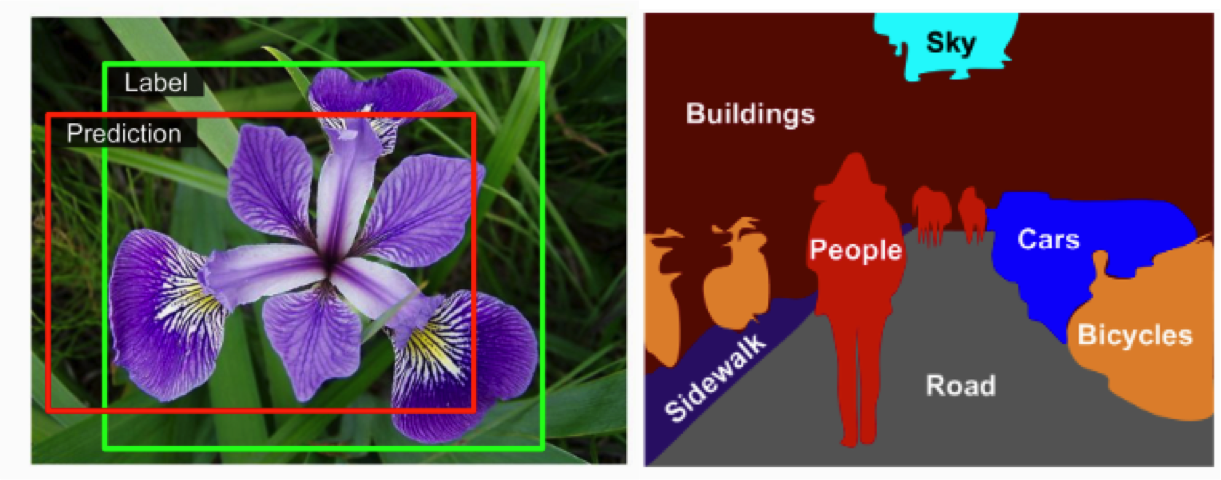
\includegraphics[width=0.9\linewidth]{figures/ch15_location.png}
\caption{Object detection (left) versus semantic segmentation (right).
Source: \citet{geron2019hands}}
\label{fig:location}
\end{figure}

It is beyond of the scope of this book to address the implementation of object detection or semantic segmentation, but we will focus on how to conduct basic image classification in state-of-the-art libraries in R and Python. As you may have imagined we will need some already-labelled images to have a proper training set. It is also out of the reach of this chapter to collect and annotate the images, which is the reason why we will mostly rely on pre-existing image databases (i.e. MINST or Fashion MINST) and pre-trained models (i.e. CNNs architectures), or will provide you with ad hoc annotated images if it is necessary. 

\subsection{Basic classification with shallow algorithms}
\label{subsec:shallow}

In Chapter~\ref{chap:introsml} we introduced you into the exciting world of machine learning and in Section~\ref{sec:supervised} we showed how to used the \textit{supervised} approach to classify texts. Most of the discussed models were based in the so called \textit{shallow} algorithms (Naïve Bayes, Regression, Support Vector Machines, Decision Trees or Random Forest), in opposition to other algorithms liked to \textit{deep} learning. As we will see in the next section, deep neural networks are nowadays the best option for complex tasks in image classification. However, we will now explain how to conduct simple multi-class classification of images that contain numbers with some shallow algorithms.

Let us begin by training a model to recognize numbers using 70,000 small images of digits handwritten from the Modified National Institute of Standards and Technology (MNIST) dataset  (\cite{lecun1998gradient}). This popular training corpus contains gray-scale examples of numbers written by American students and workers and it is usually employed to test machine learning models (60,000 for training and 10,000 for testing). Image sizes are 28 x 28, which generates 784 features for each image, with pixels values from white to black represented by a 0-255 scales. In Figure~\ref{fig:numbers} you can observe the first 10 handwritten numbers used in both training and test set.

\begin{figure}
\centering
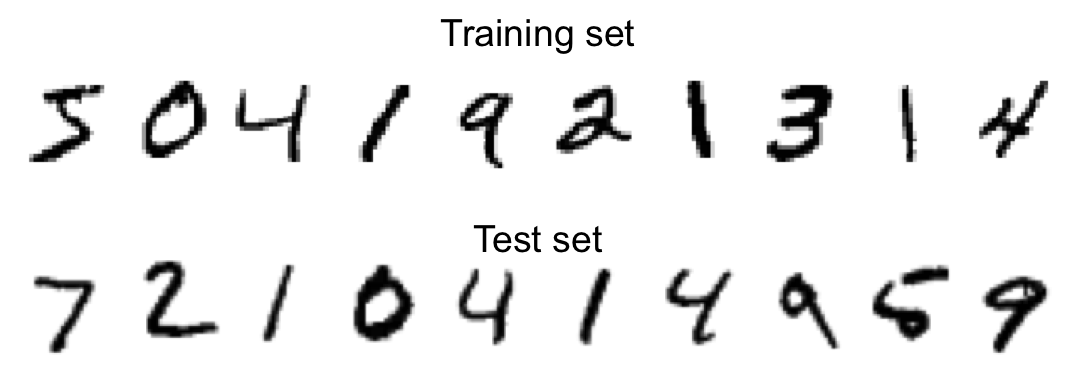
\includegraphics[width=0.9\linewidth]{figures/ch15_numbers.png}
\caption{First 10 handwritten digits from the training and test set of the MNIST}
\label{fig:numbers}
\end{figure}

You can download the MNIST images from its project web page\footnote{http://yann.lecun.com/exdb/mnist/}, but many libraries also offer this dataset. In \refex{mnist} we use the \fn{read\_mnist} function from the \pkg{dslabs} package (Data Science Labs) in R and the \fn{fetch\_openml} function from the \pkg{sklearn} package (\texttt{datasets} module) in Python to read and load a \texttt{mnist} object into our workspace. We then create the four necessary objects (\texttt{X\_train}, \texttt{X\_test}, \texttt{y\_train}, \texttt{y\_test}) to generate a ML model and print the first numbers in training and test sets and check they coincide with those in \ref{fig:numbers}.

\pyrex[output=both,caption=Loading MNIST dataset and preparing training and test sets]{chapter15/mnist}

Once we are ready to model the numbers we choose one of the shallow algorithms explained in Section \ref{sec:nb2dnn} to deploy a binary or multiclass image classification task. In the case of binary, we should select a number of reference (for instance "3") and then create the model of that number against all the others (to answer questions such as "What's the probability of this digit of being number 3?). On the other hand, if we choose multiclass classification our model can predict any of the ten numbers (0, 1, 2, 3, 4, 5, 6, 7, 8, 9) included in our examples.

Now, we used the basic concepts of the Random Forest algorithm (see subsection~\ref{subsec:randomforest}) to create and fit a model with 100 trees (\texttt{forest\_clf}). In \refex{multiclass} we use again the \pkg{randomForest} package in R and \pkg{sklearn} package in Python to estimate a model for the ten classes using the corpus of 60,000 images (classes were similarly balanced (~9-11\% each). As we do in the examples, you can check the predictions for the first ten images of the test set (\texttt{X\_test}), which correctly correspond to the right digits, and also check the (\texttt{predictions}) for the whole test set and the some metrics of the model. The accuracy is over 0.97 which is a good indicator in the classification task.

\pyrex[output=both,caption=Modeling the handwritten digits with RandomForest and predicting some outcomes]{chapter15/multiclass}

This approach based on shallow algorithms seems to work pretty well for simple images, but has a lot of limitations for more complex images such as figures or real pictures. In the next section we introduce the use of deep learning in image classification which is nowadays a more accurate approach for complex tasks.


\subsection{Deep learning for image analysis}
\label{subsec:deep}

Even when require heavy computations, Deep Neural Networks (DNN) are nowadays the best way to conduct image classification because its performance is normally higher than shallow algorithms. One of the simplest DNNs architectures is the Multilayer Perceptron (MLP) which contains one input layer, one or many hidden layers, and one output layer (all of them \textit{fully} connected and with bias neurons except for the put layer). We could also say that this is a \texttt{vanilla} neural network if we compare with more sophisticated architectures such as recurrent neural networks (RNN) or convolutional neural networks (CNN). Origginaly in a MLP the he signals propagate from the inputs to the outputs (in one direction), which we call a feedforward neural network (FNN), but using Gradient Decent as an optimizer we can apply \textit{backpropagation} (automatically computing the gradients of the network's errors in two stages: one forward and one backward) and then obtain a more efficient training.

We can use MLPs for binary and multiclass classification. In the first case, we normally use a single output neuron with the \textit{logistic} activation function (probability from 0 to 1); and in the second case we will need one output neuron per class with the \textit{softmax} activation function (probabilities from 0 to 1 for each class but they must add 1 if the classes are exclusive). To predict probabilities, in both cases we will need a \textit{loss} function and the one that is normally recommended is the \textit{cross entropy loss} or simply \textit{log loss}.

The state-of-the-art library for neural networks in general and for computer vision in particular is \pkg{TensorFlow}\footnote{We will deploy \pkg{TensorFlow} \textit{2} in our exercises.}  (originally created by Google by later publicly released) and the high-level Deep Learning API \pkg{Keras}, although you can find other good implementation packages such as \pkg{PyTorch} (created by Facebook), which has many straightforward functionalities and has also become popular in the last years (see image classification tasks for social sciences conducted in \pkg{PyTorch} by WEBB, CASAS\& WILKERSON, forthcoming XXX). All these packages have current versions for both R and Python. 

Now, let's train a MLP to build an image classifier to recognize fashion items using the Fashion MNIST dataset\footnote{https://github.com/zalandoresearch/fashion-mnist}. This dataset contains 70,000 (60,000 for training and 10,000 for test) gayscale examples (28x28) of ten different classes that include ankle boots, bags, coats, dresses, pullovers, sandals, shirts, sneakers, t-shirts/tops and trousers (Figure~\ref{fig:fashion}). If compare this dataset with the MINST we will find that figures of fashion items are more complex than handwritten digits, which normally generates a lower accuracy in supervised classification.

\begin{figure}
\centering
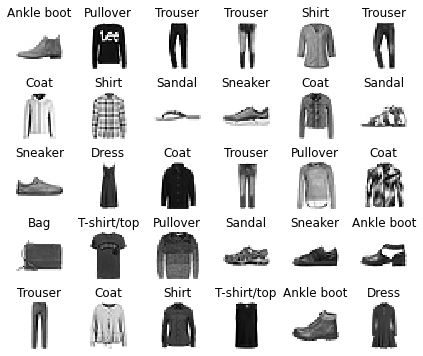
\includegraphics[width=0.9\linewidth]{figures/ch15_fashion.png}
\caption{Examples of Fashion MNIST items}.
\label{fig:fashion}
\end{figure}

You can use \pkg{Keras} to load the Fashion MNIST. In \refex{fashion} we load the complete data set and create the necessary objects for modeling (\texttt{X\_train\_full}, \texttt{y\_train\_full}, \texttt{X\_test}, \texttt{y\_test}). In addition we rescaled all the input features from 0-255 to 0-1 by dividing them by 255 in order to apply Gradient Decent. Then, we will obtain three sets with 28x28 arrays: 60,000 in the training, and 10,000 in the test. We could also generate here a validation set (e.g. \texttt{X\_valid} and \texttt{y\_valid}) with a given amount of records extracted from the training set (e.g. 5,000), but as you will later \pkg{Keras} allows us to automatically generate the validation set as a proportion of the training set (e.g. 0,1, which would be 6,000 records in our example) when fitting the model.

\pyrex[output=both,caption=Loading Fashion MNIST dataset and preparing training\, test and validation sets]{chapter15/fashion}

The next step is to design the architecture of our model. There three ways to create the models in \pkg{Keras} (\textit{sequential}, \textit{functional} or \textit{subclassing}, but the are thousands (infinite?) ways to configure a deep neural network. In the case of this MLP, we have to include first an input layer with the \texttt{input\_shape} equal to the image dimension (28x28 for 784 neurons), which is a parameter that you will easy change in other exercises (just remember that all the inputs should always have the same shape before feeding the network!). At the top of the MLP you will  need a output layer with 10 neurons (the number of posssible outcomes in out multi-class classification task) and a \textit{softmax} activation function for the final probabilities for each class.

In \refex{mlp} we use the \textit{sequential} model to design our MLP layer by layer including the above-mentioned input and output layers. In the middle, there are many options for the configuration of the \textit{hidden} layers: number of layers, number of neurons, activation functions, etc. As we know that each hidden layer will help to model different patterns of the image, it would be fair to include at least two of them with different numbers of neurons (significantly reducing this number in the second one) and transmit its information using the \textit{relu} activation function. What we actually do is to create an object called \texttt{model} which saves the proposed architecture. We can use the method \fn{summary} to obtain a clear representation of the created neural network and the number of parameter of the model (266,610 in this case!).

\pyrex[output=py,caption=Creating the architecture of the MLP with \pkg{Keras}]{chapter15/mlp}

The next steps will be to \fn{compile}, \fn{fit} and \fn{evaluate} the model, similarly to what you have already done in previous exercises of this book. In \refex{model} we first include the parameters (loss, optimizer and metrics) of the compilation step and fit the model, which might take some minutes (or even hours depending on your dataset, the architecture of you DNN and, of course, your computer). When fitting you have to separate your training set into phases or \textit{epochs} (we chose here 5 epochs, but you can increase it) and the proportion of the training set that will become the validation set (in this case 0.1). In addition, you can use the parameter \texttt{verbose} to choose weather to see the progress (1 for progress bar and 2 for one line per epoch) or not (0 for silent) of the training process. By using the method \fn{evaluate}you can then obtain the final loss and accuracy, which in this case is 0.84 (but you can reach out 0.88 if you fit it with 25 epochs!).

\pyrex[output=both,caption=Compiling\, fitting and evaluating the model for the MLP]{chapter15/model}

Finally, you can use the model to predict the classes of any new image (using \fn{predict\_classes}. In \refex{predict} we used the model to predict the classes of the first 6 elements of the test set. If you go back to \ref{fig:fashion} you can compare these predictions ('Ankle boot', 'Pullover', 'Trouser', 'Trouser', 'Shirt' and 'Trouser') with the actual first 6 images of the test set, and see how accurate our model was.

\pyrex[output=both,caption=Predicting classes using the MLP]{chapter15/predict}

Using the above-described concepts and code you may try to train a new MLP using color images of ten classes (airplane, automobile, bird, cat, deer, dog, frog, horse, ship and truck) using the CIFAR-10 and CIFAR-100 datasets\footnote{https://www.cs.toronto.edu/~kriz/cifar.html}!


\subsection{Re-using an open source CNN}
\label{subsec:tuning}

Training complex images such as photographs is normally a more sophisticated task if we compare it to the examples included in the last sections. On the one hand, it might not be a good idea to build a deep neural network from scratch as we did in subsection~\ref{subsec:deep} to train a MLP. This means that you can re-use some lowers layers of other DNNs and deploy \textit{transfer learning} to save time with less training data. On the other hand, we should also move from traditional MLPs to other kind of DNNs such as Convolutional Neural Networks (CNNs) which are  nowadays the state-of-the-art approach in computer vision. Moreover, to get good results we should also build or explore different CNNs architectures that can produce more accurate prediction in image classification.  In this section we will show how to re-use an open source CNN architecture and will suggest an example of how to fine-tune an existing CNN for a social science problem.

A CNN is a specific type of DNN that have had great success in complex visual tasks (image classification, object detection or semantic segmentation) and voice recognition\footnote{Though we recommended Recurrent Neural Networks for text classification, it is worth to mention that CNNs have also a great performance in natural language processing.}. Instead of using \textit{fully connected} layers like in a typical MLP, a CNN uses only \textit{partially connected} layers inspired on how "real" neurons connect in the visual cortex: some neurons only react to stimuli located in a limited \textit{receptive field}. In other words, in a CNN every neuron is connected to some neurons of the previous layer (and not to all of them), which significantly reduces the amount of information transmitted to the next layer and helps the DNN to detect complex patterns. Surprisingly, this reduction in the number of parameters and weights involved in the model works better for larger and more complex images, different from those shown in MNIST.

Building a CNN is quite similar to a MLP, except for the fact that you will have to work with \textit{convolutional} and \textit{pooling} layers. The convolutional layers include a \textit{bias term} and are the most important blocks of a CNN because they establish the specific connections  among the neurons. In simpler words: a given neuron of an high-level layer is connected only to a rectangular group of neurons (the receptive field) of the low-level layer and not to all of them. If the input layer (in the case of colour images there are three sublayers, one per color channel) and the convolutional layers are of different sizes we can apply techniques such as \textit{zero padding} (adding zeros around the inputs) or spacing out the receptive fields (each shift from one receptive field to the other will be a \textit{stride}). In order to transmit the weights from the receptive fields to the neurons, the convolutional layer will automatically generate some \textit{filters} to create \textit{features maps}, which are the areas of the input that mostly active those filters. Additionally, by creating subsamples of the inputs, the pooling layers will reduce the number of parameters, the computational effort of the network and the risk of overfitting. The pooling layers \textit{aggregates} the inputs using a standard arithmetic function such as minimum, maximum or mean. For more technical details of the basis of a CNN you can can go to specific literature such as \cite{geron2019hands}.

Instead of building a CNN from scratch, there are many pre-trained and open-source architectures that have been optimized for image classification. Besides a stack of convolutional and pooling layers,  these architectures normally include some fully connected layers and a regular output layer for prediction (just like in MLPs). We can mention some of these architectures: LeNet-5, AlexNet, GoogLeNet, VGGNet, ResNet, Xception or SENet\footnote{The description of technical details of all of these architectures are out of the scope of this book, but besides the specific scientific literature of each architecture, some packages such as \pkg{keras} usually include basic documentation.}. All these CNNs have been previously tested in image classification with promising results, but you still have to look at the internal composition of each of them and their metrics to choose the most appropriate for you. You can implement and train most them from scratch either in \pkg{keras} or \pkg{PyTorch}, or you can just use them directly or even fine-tune the pretrained model in order to save time. 

Let's use the pre-trained model of a Residual Network (ResNet) with 50 layers, also known as \textit{ResNet50}, to show you how to deploy a multi-class classifier over pictures. The ResNet architecture (also with 34, 101 and 152 layers) is based on the so called residual learning and uses \textit{skip connections}, which means that the input layer does not only feed the next layer but this signal is also added to the output of another high-level layer. This allows you to have a much deeper network and in the case of ResNet152 it has achieved a top-five error rate of 3.6\%. As we do in \refex{resnet50}, you can easily import onto your workspace a ResNet50 architecture and include the pre-trained weights of a model trained with ImageNet (uncomment the second line of the code to visualize the complete model!).

\pyrex[output=none,caption=Loading a visualizing the ResNet50 architecture]{chapter15/resnet50}

ImageNet is a corpus of labelled images based on the WordNet hierarchy. ResNet uses a subset of ImageNet with \~1,000 examples for each of the 1,000 classes for a total corpus of roughly 1,350,000 pictures (1,200,000 for training, 100,000 for test, and 50,000 for validation).

In \refex{newimages} we crop a part of our second example picture of refugees arriving to the European costs (\texttt{my\_image2\_RGB}) in order to get just the sea landscape. With the created \texttt{model\_resnet50} we then ask up to three predictions of the class of the photograph in \refex{resnetpredictions}.

\pyrex[output=both,format=png,caption=Cropping an image to get a picture of a see landscape]{chapter15/newimages}

\pyrex[output=both,caption=Predicting the class of the first image]{chapter15/resnetpredictions}

As you can see in the Python and R outputs\footnote{Outputs in Python and R might differ a little bit since the crops for the new images were similar but not identical.}, the best guest of the model is a \textit{sandband}, which is very close to the real picture that contains see water, mountains and sky. However, it seems that the model is confusing sand with see. Other results in the Python model are \textit{seashore} and \textit{cliff}, which are also very close to real see landscape. Neverthelss, in the case of the R prediction the model detects a \textit{submarine} and a \textit{gray whale}, which revels that predictions are not 100\% accurate yet.

If we do the same with another part of that original picture and focus only on the  group of refugees over a lifeboat while arriving to the European coast, we will get a different result! In \refex{newimages2} we crop again (\texttt{my\_image2\_RGB}) and get a new framed picture. Then in \refex{resnetpredictions2} we re-run the prediction task using the model \textit{ResNet50} trained with ImageNet and get a very nice accurate result: Both predictions coincide to see a \textit{lifeboat}, which is a very good tag for the image we want to classify. Again, other lower-level predictions can seem accurate (\textit{speepboad}) and totally inaccurate (\textit{vulcano}, \textit{gray whale} or \textit{amphibian}).

\pyrex[output=both,format=png,caption=Cropping an image to get a picture of refugees in a lifeboat]{chapter15/newimages2}

\pyrex[output=both,caption=Predicting the class of the second image]{chapter15/resnetpredictions2}

These examples show you how to use directly an open-source and pre-trained CNN that has 1,000 classes and has been trained on images that we do not have control of. However, you may want to build your own classifier with your own training data, but using part of an existing architecture. This is called fine-tuning and you can follow a good example in social science in WEBB, CASAS\& WILKERSON (forthcoming XXX). The authors re-use RestNet18 to build binary and multi-class classifiers adding their own data examples over the pre-trained CNN\footnote{The examples are provided in Python with the package \pkg{PyTorch}, which is quite friendly if you are already familiar to \pkg{Keras} }. For example, in a binary classification, they use pictures related to the \textit{BlackLiveMatters} movement to model if a picture is a protest or not (99 true positives and 100 true negatives). This is an excellent example of how you can adapt image classification tasks to answer specific research questions in social sciences.